\documentclass[fleqn]{article}

\usepackage[utf8]{inputenc}
\usepackage{amsmath}
\usepackage{graphicx}
\usepackage{bm}
\usepackage[margin=0.75in]{geometry}

\newcommand*\diff{\mathop{}\!\mathrm{d}}
\newcommand*\Diff[1]{\mathop{}\!\mathrm{d^#1}}
\newcommand{\cnum}{ECE 141 COVID-19 Project}
\newcommand{\ced}{Spring 2020}

\begin{document}

\title{ECE 141 COVID-19 Project}
\author{Comran Morshed (SID: 404544982, Discussion 1D)}
\date{}
\maketitle

\section*{Problem 1}
Based on the results of the simulation (shown below), it appears that an overwhelming majority of the population became infected -- causing about 14\% of people to die. There also appears to be a peak infection that is quickly reached around $t=25$, which ultimately decays as more individuals settle into either the recovered or dead group.

\begin{center}
    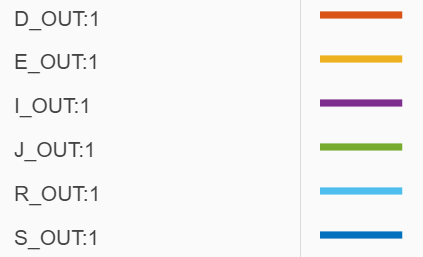
\includegraphics[width=4cm]{outbreak_legend} \\
    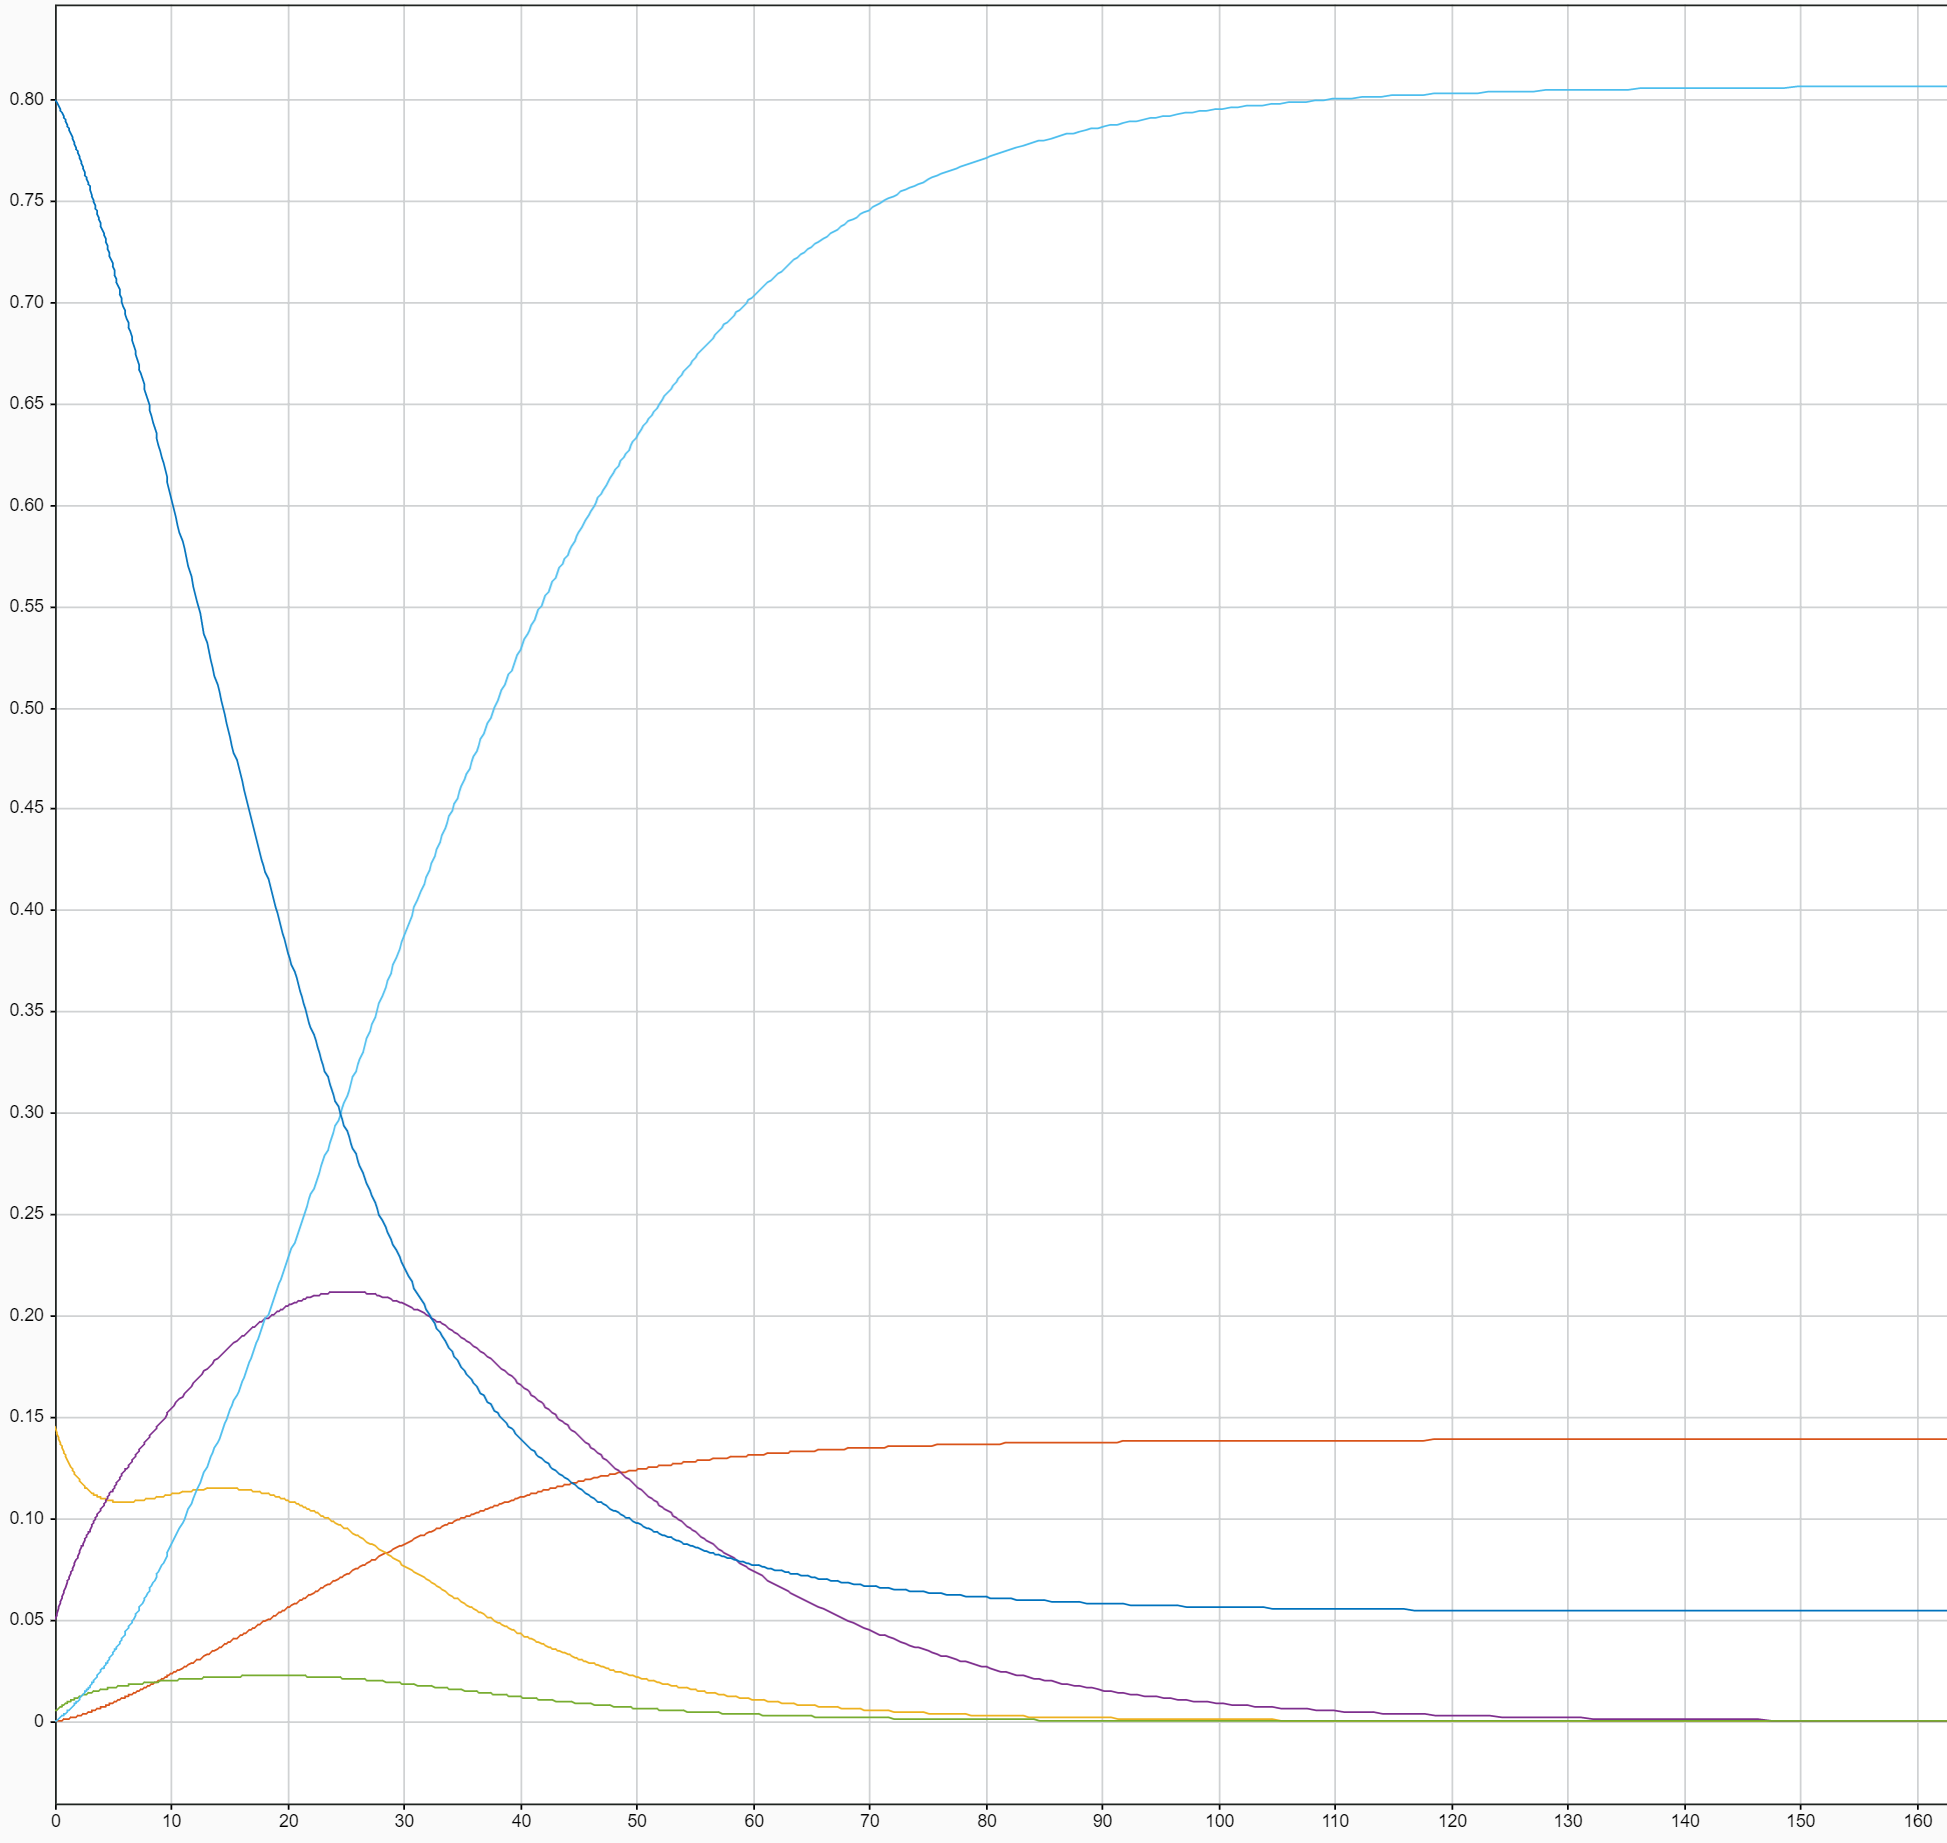
\includegraphics[width=0.85\linewidth]{outbreak_graph}
\end{center}

\newpage

\subsection*{Nonlinear Laplace transforms}
$sS(s) = -\beta_1 S I(s) - \beta_2 S J(s) + S(0)$ \\
$sE(s) = \beta_1 S I(s) + \beta_2 S J(s) - \gamma E(s) + E(0)$ \\
$sI(s) = \sigma_1 \gamma E(s) - \rho_1 I(s) + I(0)$ \\
$sJ(s) = \sigma_2 \gamma E(s) - (\rho_2 + q) J(s) + J(0)$ \\
$sR(s) = \rho_1 I(s) + \rho_2 J(s) + R(0)$ \\
$sD(s) = qJ(s) + D(0)$ \\

\subsection*{Simulink diagram for nonlinear model}
\begin{center}
    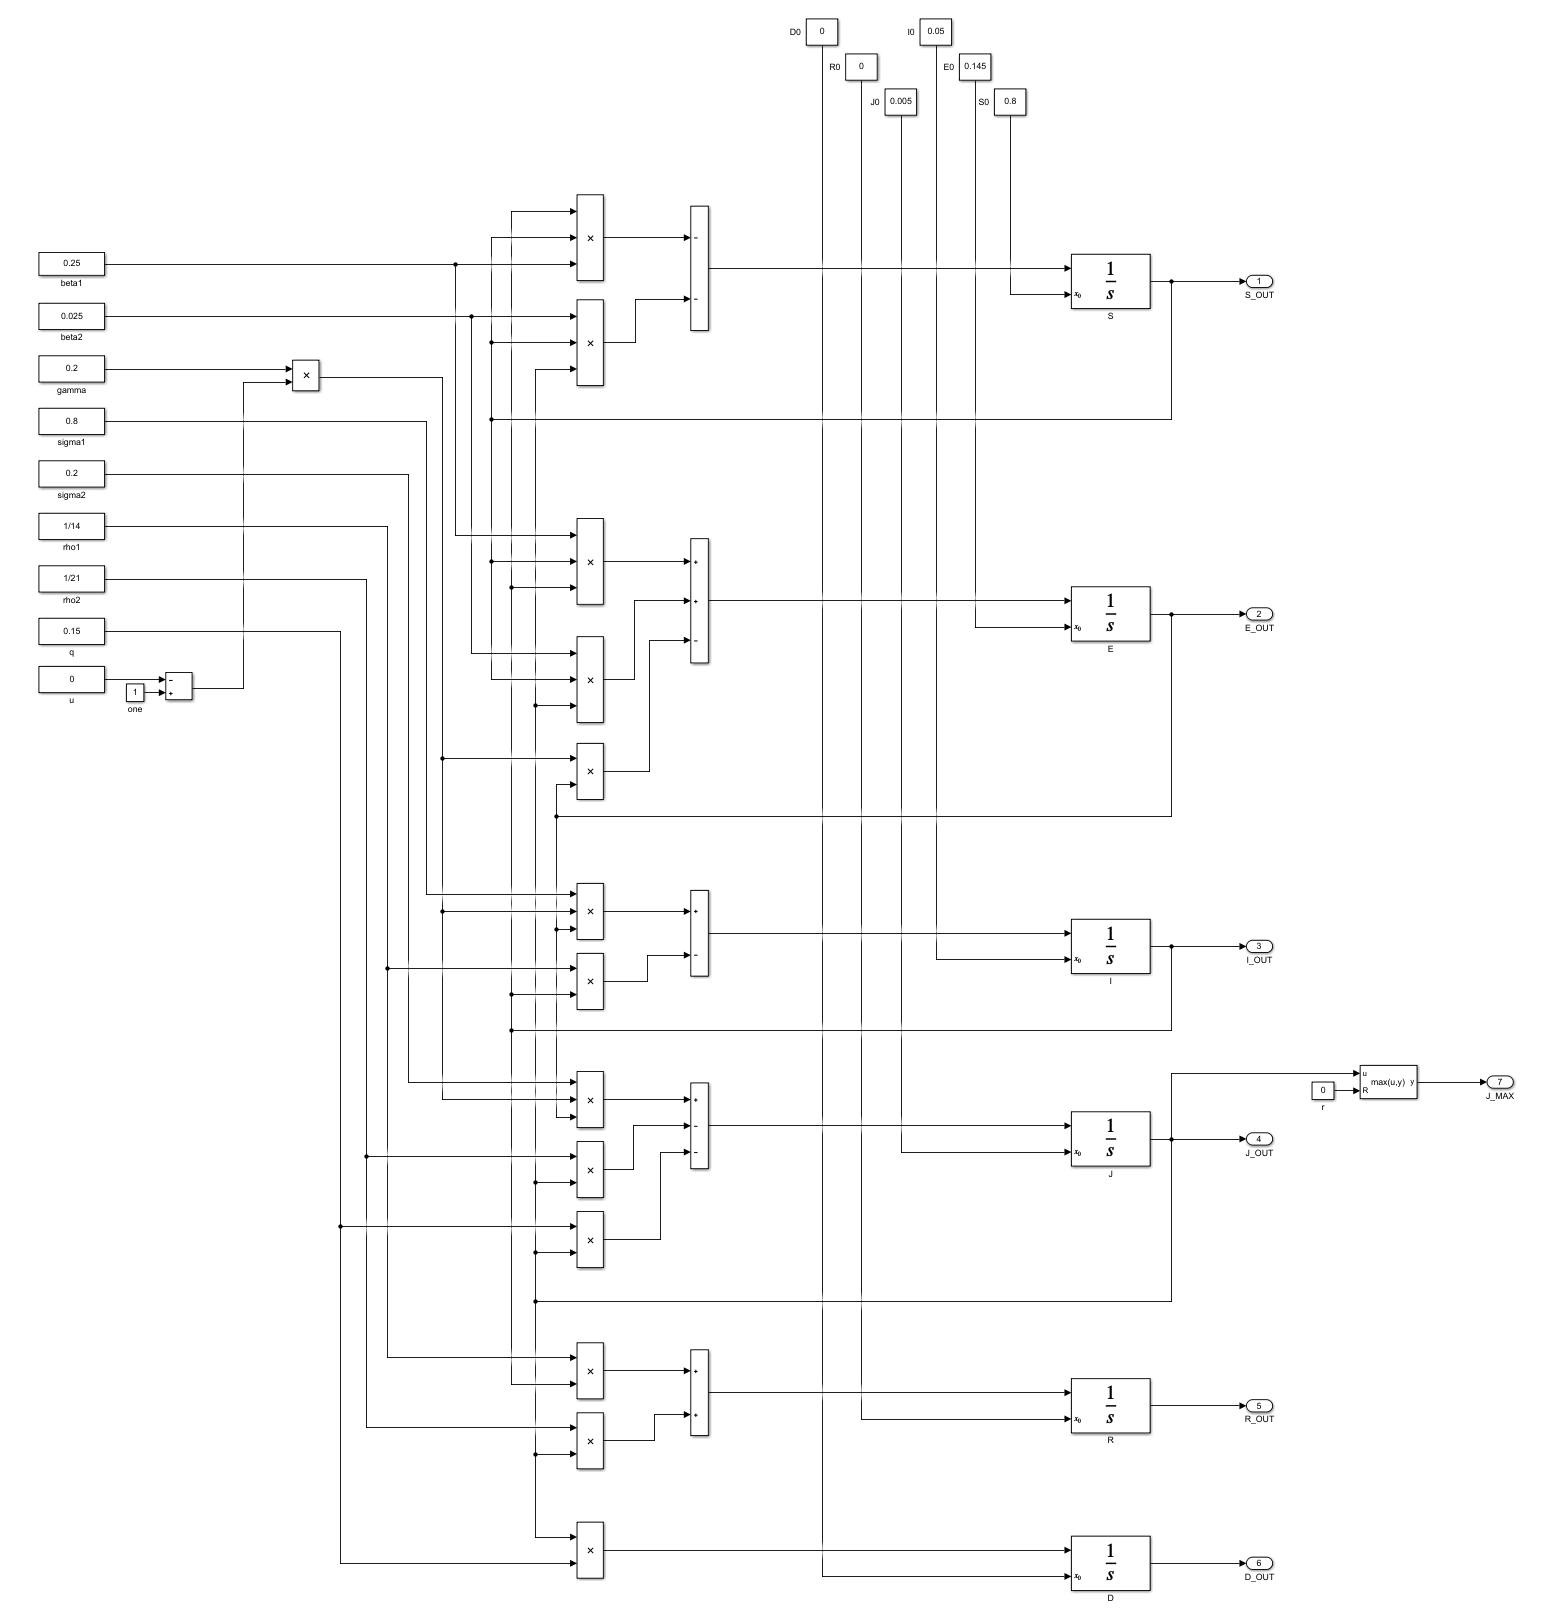
\includegraphics[width=\linewidth]{simulink_diagram}
\end{center}

\newpage

\section*{Problem 2}
There will need to be enough hospital beds to support \textbf{2.25\%} of the population at the peak of the outbreak. This was determined by creating a new signal containing the maximum value of individuals that are seriously ill, and checking the maximum value after the simulation has reached steady state. This is more than twice the percentage of hospital beds available for this population, so there will ultimately be seriously ill individuals who cannot be treated by the overwhelmed hospital system (which, in addition, may have an even lower treatment capabilities as doctors and nurses also become infected).
\begin{center}
    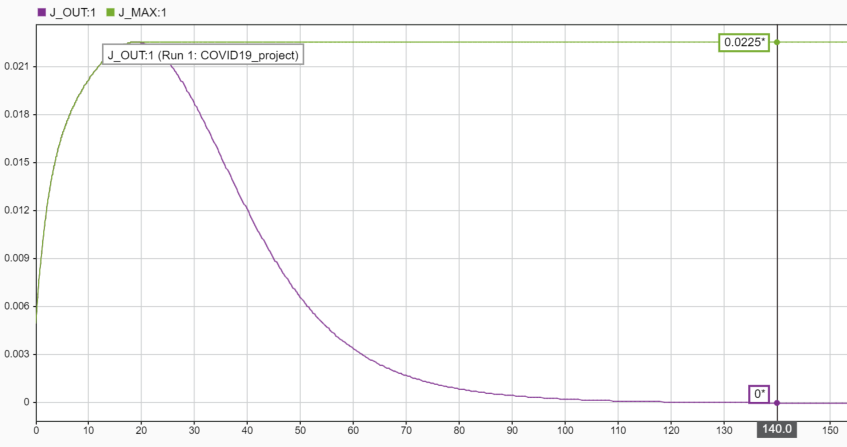
\includegraphics[width=\linewidth]{simulink_J_max}
\end{center}

\newpage
\section*{Problem 3}
\subsection*{Linearization}
\begin{equation*}
    \bm{x} = \begin{bmatrix}
        x_1 \\
        x_2 \\
        x_3 \\
        x_4 \\
        x_5 \\
        x_6
    \end{bmatrix} = \begin{bmatrix}
        S \\
        E \\
        I \\
        J \\
        R \\
        D
    \end{bmatrix}
\end{equation*}

\begin{equation*}
    A = \dfrac{\diff f}{\diff x} \bigg\rvert_{\bm{x_e}, \bm{u_e}}
\end{equation*}

\begin{equation*}
    B = \dfrac{\diff f}{\diff u} \bigg\rvert_{\bm{x_e}, \bm{u_e}}
\end{equation*}

Plug in the model used for this project.

\begin{equation*}
    \begin{split}
        \dfrac{\diff}{\diff t} \diff x & = \bm{A} \diff x + \bm{B} \diff u \bigg\rvert_{\bm{x_e}, \bm{u_e}} \\
            & = \begin{bmatrix}
                0 & 0 & {-\beta_1 S_e} & {-\beta_2 S_e} & 0 & 0 \\
                0 & -(1 - u_e) \gamma & {\beta_1 S_e} & {\beta_2 S_e} & 0 & 0 \\
                0 & (1 - u_e) \sigma_1 \gamma & -\rho_1 & 0 & 0 & 0 \\
                0 & (1 - u_e) \sigma_2 \gamma & 0 & -(\rho_2 + q) & 0 & 0 \\
                0 & 0 & \rho_1 & \rho_2 & 0 & 0 \\
                0 & 0 & 0 & q & 0 & 0 \\
            \end{bmatrix} \cdot \begin{bmatrix}
                \diff S \\
                \diff E \\
                \diff I \\
                \diff J \\
                \diff R \\
                \diff D
            \end{bmatrix} + \begin{bmatrix}
                0 \\
                \gamma E_e \\
                -\sigma_1 \gamma E_e \\
                -\sigma_q \gamma E_e \\
                0 \\
                0
            \end{bmatrix} \diff u
    \end{split}
\end{equation*}


\subsection*{Equilibrium pair}
Need to find an equilibrium pair s.t. $f(x_e, u_e) = 0$.

\begin{equation*}
    \begin{split}
        \begin{bmatrix}
            0 \\
            0 \\
            0 \\
            0 \\
            0 \\
            0 \\
        \end{bmatrix} & = \begin{bmatrix}
            0 & 0 & {-\beta_1 S_e} & {-\beta_2 S_e} & 0 & 0 \\
            0 & -(1 - u_e) \gamma & {\beta_1 S_e} & {\beta_2 S_e} & 0 & 0 \\
            0 & (1 - u_e) \sigma_1 \gamma & -\rho_1 & 0 & 0 & 0 \\
            0 & (1 - u_e) \sigma_2 \gamma & 0 & -(\rho_2 + q) & 0 & 0 \\
            0 & 0 & \rho_1 & \rho_2 & 0 & 0 \\
            0 & 0 & 0 & q & 0 & 0 \\
        \end{bmatrix} \cdot \begin{bmatrix}
            S_e \\
            E_e \\
            I_e \\
            J_e \\
            R_e \\
            D_e
        \end{bmatrix} + \begin{bmatrix}
            0 \\
            \gamma E_e \\
            -\sigma_1 \gamma E_e \\
            -\sigma_q \gamma E_e \\
            0 \\
            0
        \end{bmatrix} u_e \\
        & = \begin{bmatrix}
            0 & 0 & {-\beta_1 S_e} & {-\beta_2 S_e} & 0 & 0 \\
            0 & -(1 - u_e) \gamma & {\beta_1 S_e} & {\beta_2 S_e} & 0 & 0 \\
            0 & (1 - u_e) \sigma_1 \gamma & -\rho_1 & 0 & 0 & 0 \\
            0 & (1 - u_e) \sigma_2 \gamma & 0 & -(\rho_2 + q) & 0 & 0 \\
            0 & 0 & \rho_1 & \rho_2 & 0 & 0 \\
            0 & 0 & 0 & q & 0 & 0 \\
        \end{bmatrix} \cdot \begin{bmatrix}
            S_e \\
            0 \\
            0 \\
            0 \\
            R_e \\
            D_e
        \end{bmatrix} + \begin{bmatrix}
            0 \\
            \gamma \cdot 0 \\
            -\sigma_1 \gamma \cdot 0 \\
            -\sigma_q \gamma \cdot 0 \\
            0 \\
            0
        \end{bmatrix} \cdot u_e
    \end{split}
\end{equation*}

Therefore,
\begin{equation*}
    \begin{bmatrix}
        S_e \\
        E_e \\
        I_e \\
        J_e \\
        R_e \\
        D_e
    \end{bmatrix} = \begin{bmatrix}
        S_e \\
        0 \\
        0 \\
        0 \\
        R_e \\
        D_e
    \end{bmatrix}
\end{equation*}

\subsection*{Final linearized form}
\begin{equation*}
    \dfrac{\diff x}{\diff t} = \begin{bmatrix}
        0 & 0 & {-\beta_1 S_e} & {-\beta_2 S_e} & 0 & 0 \\
        0 & -(1 - u_e) \gamma & {\beta_1 S_e} & {\beta_2 S_e} & 0 & 0 \\
        0 & (1 - u_e) \sigma_1 \gamma & -\rho_1 & 0 & 0 & 0 \\
        0 & (1 - u_e) \sigma_2 \gamma & 0 & -(\rho_2 + q) & 0 & 0 \\
        0 & 0 & \rho_1 & \rho_2 & 0 & 0 \\
        0 & 0 & 0 & q & 0 & 0 \\
    \end{bmatrix} \cdot \begin{bmatrix}
        \diff S \\
        \diff E \\
        \diff I \\
        \diff J \\
        \diff R \\
        \diff D
    \end{bmatrix} + \begin{bmatrix}
        0 \\
        0 \\
        0 \\
        0 \\
        0 \\
        0
    \end{bmatrix} \diff u
\end{equation*}

\begin{equation*}
    \bm{A} = \begin{bmatrix}
        0 & 0 & {-\beta_1 S_e} & {-\beta_2 S_e} & 0 & 0 \\
        0 & -(1 - u_e) \gamma & {\beta_1 S_e} & {\beta_2 S_e} & 0 & 0 \\
        0 & (1 - u_e) \sigma_1 \gamma & -\rho_1 & 0 & 0 & 0 \\
        0 & (1 - u_e) \sigma_2 \gamma & 0 & -(\rho_2 + q) & 0 & 0 \\
        0 & 0 & \rho_1 & \rho_2 & 0 & 0 \\
        0 & 0 & 0 & q & 0 & 0 \\
    \end{bmatrix}
\end{equation*}

\begin{equation*}
    \bm{B} = \begin{bmatrix}
        0 \\
        0 \\
        0 \\
        0 \\
        0 \\
        0
    \end{bmatrix}
\end{equation*}

Pick equilibrium values that are expected at the end of the pandemic.
\begin{equation*}
    \begin{bmatrix}
        S_e \\
        R_e \\
        D_e
    \end{bmatrix} = \begin{bmatrix}
        0.0542 \\
        0.807 \\
        0.139
    \end{bmatrix}
\end{equation*}

\begin{equation*}
    u_e = 0
\end{equation*}

\subsection*{Linear Laplace transforms}
$sS(s) = -\beta_1 S_e I(s) - \beta_2 S_e J(s) + S(0)$ \\
$sE(s) = \beta_1 S_e I(s) + \beta_2 S_e J(s) - (1-u_e) \gamma E(s) + E(0)$ \\
$sI(s) = (1-u_e) \sigma_1 \gamma E(s) - \rho_1 I(s) + I(0)$ \\
$sJ(s) = (1-u_e) \sigma_2 \gamma E(s) - (\rho_2 + q) J(s) + J(0)$ \\
$sR(s) = \rho_1 I(s) + \rho_2 J(s) + R(0)$ \\
$sD(s) = qJ(s) + D(0)$ \\

\newpage

\subsection*{Linearized simulation}
\begin{center}
    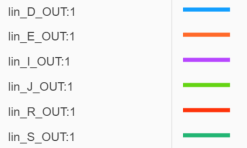
\includegraphics[width=4cm]{linear_outbreak_legend} \\
    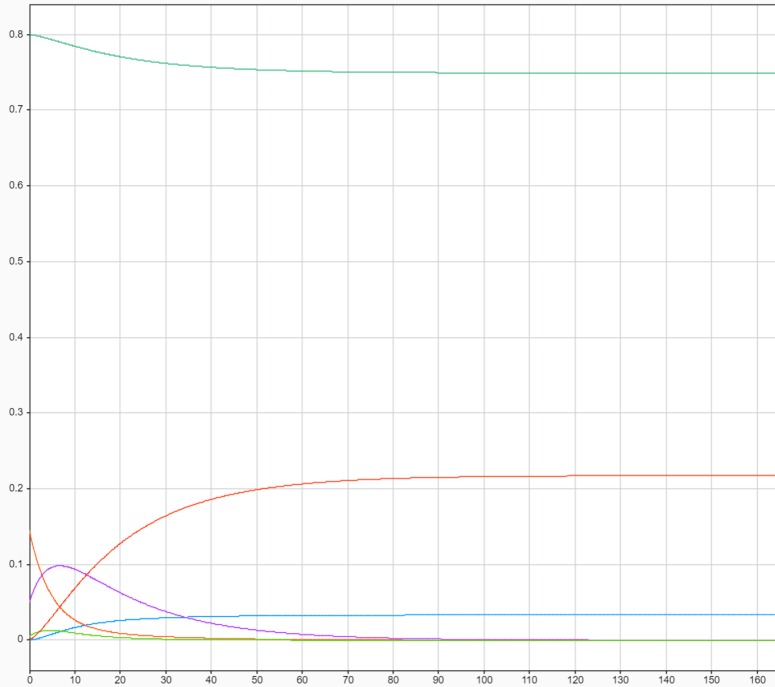
\includegraphics[width=0.85\linewidth]{linear_outbreak_graph}
\end{center}

\newpage

\subsection*{Simulink diagram for linear model}
\begin{center}
    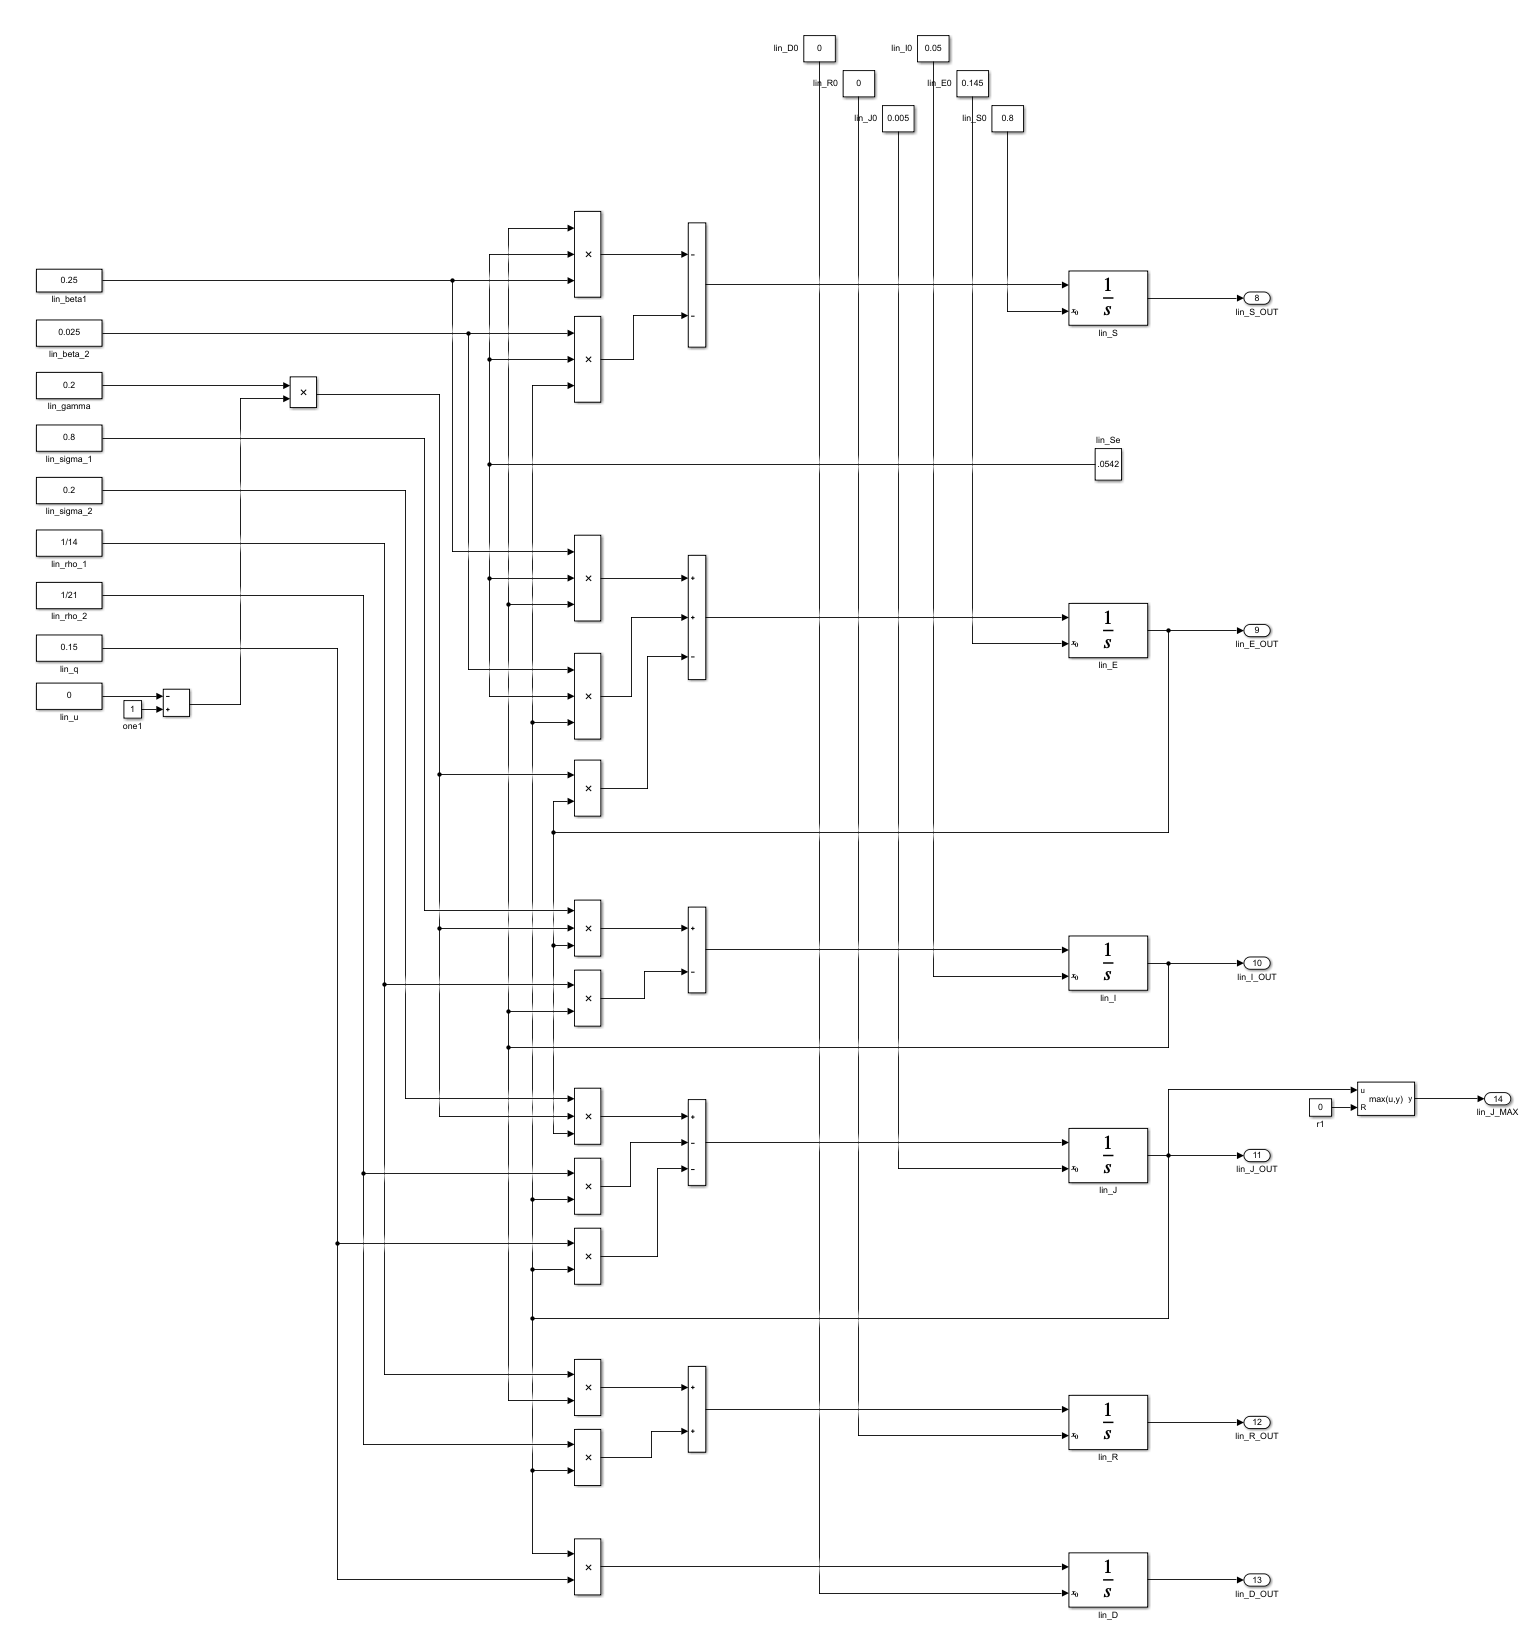
\includegraphics[width=\linewidth]{linear_simulink_diagram}
\end{center}

\subsection*{Issue with the linearized model}
This linearized model would not be adequate for control since it assumes a constant value for $S_e$. In reality, this value is much higher at the beginning of the pandemic than at the end as the population becomes immune to the disease.

\section*{Problem 4}
\subsection*{Find a transfer function from J(0) $\rightarrow$ J}

$sJ(s) = (1-u_e) \sigma_2 \gamma E(s) - (\rho_2 + q) J(s) + J(0)$ \\
$J(s)(s + \rho_2 + q) = (1-u_e) \sigma_2 \gamma E(s) + J(0)$ \\
$J(s) = \dfrac{(1-u_e) \sigma_2 \gamma E(s) + J(0)}{s + \rho_2 + q}$ \\
$J(s) = \dfrac{(1-u_e) \sigma_2 \gamma}{s + \rho_2 + q} E(s) + \dfrac{J(0)}{s + \rho_2 + q}$ \\
\\
\\
$sE(s) = \beta_1 S_e I(s) + \beta_2 S_e J(s) - (1-u_e) \gamma E(s) + E(0)$ \\
$E(s)(s + (1-u_e) \gamma) = \beta_1 S_e I(s) + \beta_2 S_e J(s) + E(0)$ \\
\\
$sI(s) = (1-u_e) \sigma_1 \gamma E(s) - \rho_1 I(s) + I(0)$ \\
$I(s)(s + \rho_1) = (1-u_e) \sigma_1 \gamma E(s) + I(0)$ \\
$I(s) = \dfrac{(1-u_e) \sigma_1 \gamma E(s) + I(0)}{s + \rho_1}$ \\
\\
\\
Set $E(0) = 0$, $I(0) = 0$: \\
$E(s)(s + (1-u_e) \gamma) = \dfrac{\beta_1 \sigma_1 \gamma S_e (1-u_e)}{s + \rho_1} E(s) + \beta_2 S_e J(s)$ \\
$E(s)\left(s + (1-u_e) \gamma - \dfrac{\beta_1 \sigma_1 \gamma S_e (1-u_e)}{s + \rho_1}\right) = \beta_2 S_e J(s)$ \\
$E(s) = \dfrac{\beta_2 S_e (s + \rho_1)}{s (s + \rho_1) + (1-u_e) (s + \rho_1) \gamma - \beta_1 \sigma_1 \gamma S_e (1-u_e)} J(s)$ \\

\begin{equation*}
\begin{split}
J(s) & = \dfrac{(1-u_e) \sigma_2 \gamma}{s + \rho_2 + q} \dfrac{\beta_2 S_e (s + \rho_1)}{s (s + \rho_1) + (1-u_e) (s + \rho_1) \gamma - \beta_1 \sigma_1 \gamma S_e (1-u_e)} J(s) + \dfrac{J(0)}{s + \rho_2 + q} \\
    & = \dfrac{\beta_2 S_e \sigma_2 \gamma (1-u_e)(s + \rho_1)}{s (s + \rho_1) + (1-u_e) (s + \rho_1) \gamma - \beta_1 \sigma_1 \gamma S_e (1-u_e)} J(s) + \dfrac{J(0)}{s + \rho_2 + q}
\end{split}
\end{equation*}

\begin{equation*}
\begin{split}
J(s)\left(1 - \dfrac{\beta_2 S_e \sigma_2 \gamma (1-u_e)(s + \rho_1)}{s (s + \rho_1) + (1-u_e) (s + \rho_1) \gamma - \beta_1 \sigma_1 \gamma S_e (1-u_e)}\right) & = \dfrac{J(0)}{s + \rho_2 + q}
\end{split}
\end{equation*}

\begin{equation*}
\begin{split}
\dfrac{J(s)}{J(0)} & = \dfrac{1}{\left(1 - \dfrac{\beta_2 S_e \sigma_2 \gamma (1-u_e)(s + \rho_1)}{s (s + \rho_1) + (1-u_e) (s + \rho_1) \gamma - \beta_1 \sigma_1 \gamma S_e (1-u_e)}\right)(s + \rho_2 + q)} \\
    & = \dfrac{1}{(s + \rho_2 + q) - \dfrac{\beta_2 S_e \sigma_2 \gamma (1-u_e)(s + \rho_1)(s + \rho_2 + q)}{s (s + \rho_1) + (1-u_e) (s + \rho_1) \gamma - \beta_1 \sigma_1 \gamma S_e (1-u_e)}} \\
    & = \dfrac{s (s + \rho_1) + (1-u_e) (s + \rho_1) \gamma - \beta_1 \sigma_1 \gamma S_e (1-u_e)}{(s + \rho_2 + q)(s (s + \rho_1) + (1-u_e) (s + \rho_1) \gamma - \beta_1 \sigma_1 \gamma S_e (1-u_e)) - \beta_2 S_e \sigma_2 \gamma (1-u_e)(s + \rho_1)(s + \rho_2 + q)} \\
    & = \dfrac{s^2 + (\rho_1 + \gamma + \rho_1 \gamma - u_e \gamma - \rho_1 u_e \gamma) s - \beta_1 \sigma_1 \gamma S_e (1-u_e)}{(s + \rho_2 + q)(s^2 + (\rho_1 + \gamma + \rho_1 \gamma - u_e \gamma - \rho_1 u_e \gamma) s - \beta_1 \sigma_1 \gamma S_e (1-u_e) - \beta_2 S_e \sigma_2 \gamma (1-u_e)(s + \rho_1))} \\
    & = \dfrac{s^2 + (0.285714 - 0.214286 u_e)s - 0.002168 (1 - u_e)}{s^3 + (0.468993 - 0.199946 u_e) s^2 + (0.0657426 - 0.0516269 u_e) s + 0.00239393 (1 - u_e)}
\end{split}
\end{equation*}

\newpage

\subsection*{Root locus}
When setting $u_e = 0$, the transfer function has the following root locus:
\begin{center}
    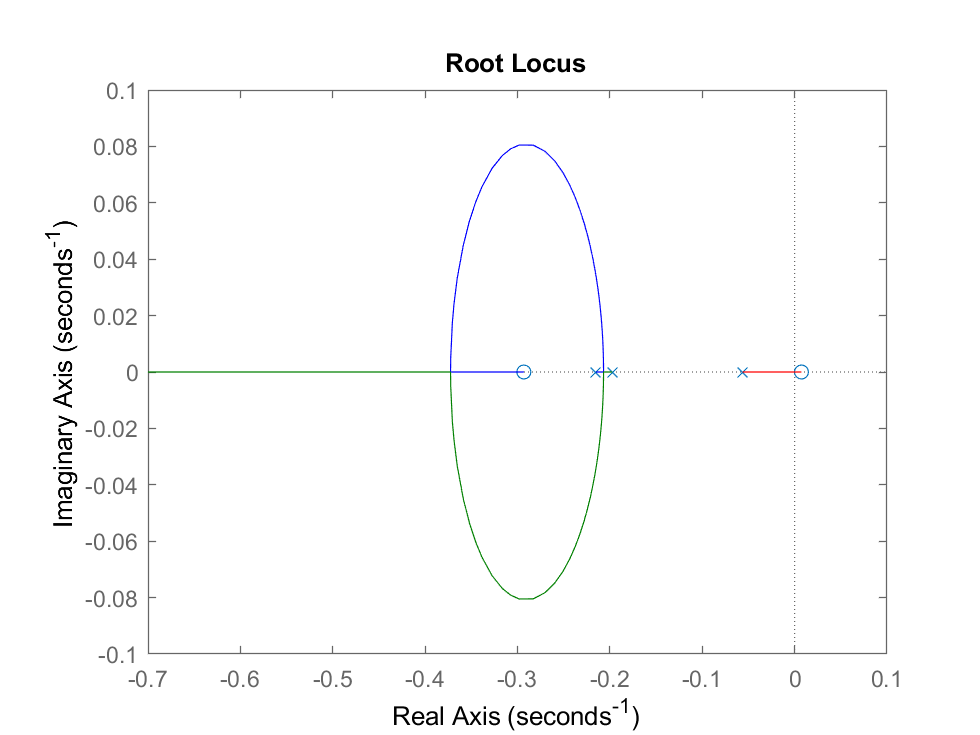
\includegraphics[width=0.7\linewidth]{tf_root_locus_u_0}
\end{center}

Additionally, when setting $u_e = 0.9$, the transfer function has the following root locus:
\begin{center}
    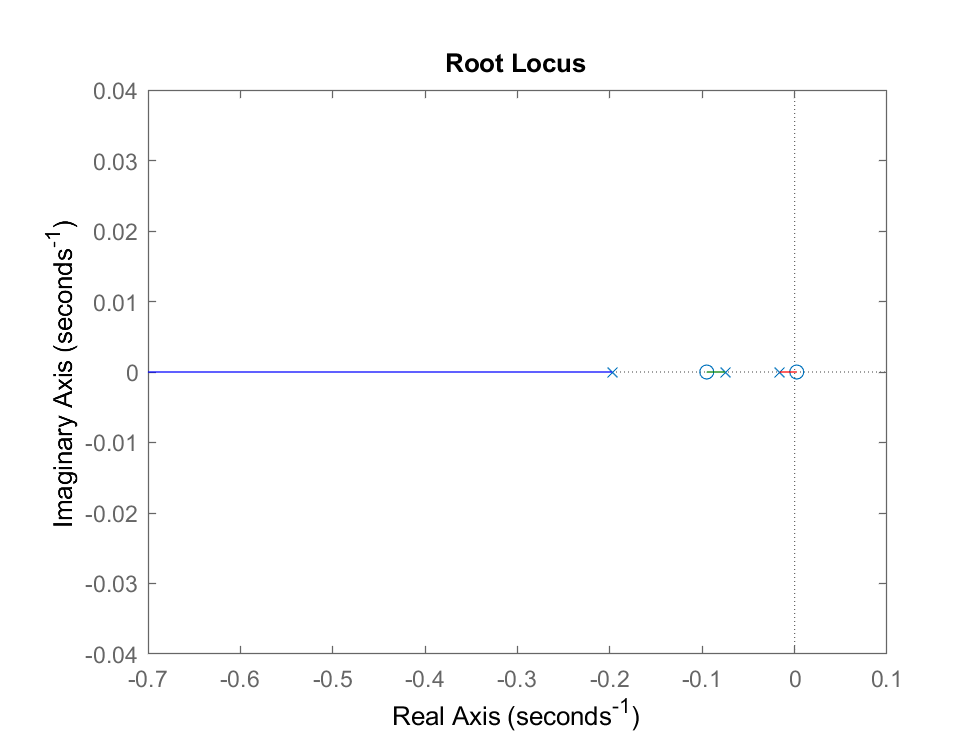
\includegraphics[width=0.7\linewidth]{tf_root_locus_u_0_9}
\end{center}

There are three poles and two zeros in the transfer function, and \textbf{all of the zeros are on the real axis}. However, for $u_e = 0.9$, the poles are closer to zero. After testing with other values, it appears that \textbf{higher values for $u_e$ result in a shifting of the poles towards zero}. This would result in a quicker decay of the number of patients requiring critical treatment (classified by variable J) and, therefore, a lower strain on the hospital system. Since wearing masks would logically slow the spread of the disease, it makes intuitive sense that the stress on the hospital system would also decay faster.

\newpage

\subsection*{Simulink model comparing values of u}

Comparing different values for u in my linear Simulink model supports the conclusion made for this transfer function. In addition, it is apparent that the system shows signs of underdamping for lower values of $u_e$. Although such a system reaches zero sooner, the initial overshoot has the potential to overload the hospital system with critically ill patients. By increasing u, the overshoot begins to disappear and, for the maximal possible value of $u_e = 0.9$, the system begins to resemble a more desirable critically-damped signal.

\begin{center}
    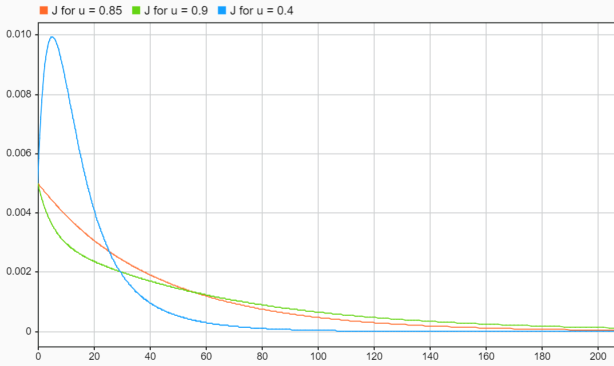
\includegraphics[width=\linewidth]{comparison_of_u_values_simulink}
\end{center}

\newpage

\section*{Problem 5}

\section*{Problem 6}

\section*{Problem 7}

\end{document}
